\documentclass[8pt]{beamer}
\usetheme{Darmstadt}
\usefonttheme{professionalfonts}
\usepackage{kotex,animate,tikz}
\title{Dispersion for the Schr\"odinger Equation}
\author{최익한}

\setlength{\parindent}{1em}

\usepackage{mypackage}

\begin{document}
\maketitle
% Some macros
\def\Fconst{\frac1{\sqrt{2\pi}^d}}
\def\qed{\hfill$\qedsymbol$}
\let\emph\relax
\NewDocumentCommand{\emph}{+m}{\textit{\textbf{#1}}}



\begin{frame}
\tableofcontents
\end{frame}
\begin{frame}
Warning:
Almost every proof is not mathematically valid!!
\end{frame}

\section{What is dispersion?}

\begin{frame}
\frametitle{1.1. Optics}
A simplest wave in $d$-dimensional space can be written in the form
\[\psi(t,\vec{x})=A\sin(\vec{k}\.\vec{x}-\omega t).\]
${}$ There are several terminologies.
\begin{itemize}
\item Amplitude $A$
\item Angular frequency $\omega=2\pi f$
\item Wave number $\vec{k}$ : \emph{vector} with direction of light propagation and size $2\pi/\lambda$
\end{itemize}
${}$
This is a solution of ``wave equation''
\[\pd[2]{t}\psi(t,\vec{x})=v^2\pd[2]{\vec{x}}\psi(t,\vec{x}),\]
which describes waves of \emph{constant velocity} $v=\omega/|\vec{k}|$.
\end{frame}

\begin{frame}
\frametitle{1.1. Optics}
The \emph{index of refraction} is defined as
\[n:=\frac c{v_p}=\frac c{\omega/|\vec{k}|}.\]
Here $\omega$ and $\vec{k}$ are measured in a transparent material.
\begin{center}\includegraphics[width=0.3\textwidth]{prism}\end{center}
${}$ \emph{Dispersion} is the phenomenon of optics that
\[\text{\emph{the index of refraction depends on wavelength.}}\] 
${}$ In other words, we have
\[\frac\omega{|\vec{k}|}\ne\text{const with respect to }\vec{k},\]
which means the relation between $\omega$ and $\vec{k}$ is not like the solutions of the wave equation.
\end{frame}

\begin{frame}
\frametitle{1.2. Dispersion relation}
\begin{defn}[Dispersion relation]
Dispersion relation is a function $\omega=\omega(\vec{k})$ which describes the relation between angular frequency $\omega\in\R$ and the wave number vector $\vec{k}\in\R^d$.
\end{defn}
${}$ Many physics can be described by language of waves and dispersion relations.\\[1em]
\textbf{Example.}
\[\text{Cauchy's formula: dispersion relation of light in transparent materials.}\]
${}$
\[\arraycolsep1.4pt\renewcommand{\arraystretch}{1.5}\begin{array}{crl}
\text{ordinary wave:}\qquad & \omega&=v|\vec{k}|\\
\text{advection:}\qquad & \omega&=\vec{v}\.\vec{k}\\
\text{heat distribution:}\qquad & \omega&=i\alpha|\vec{k}|^2\\
\text{quantum mechanics:}\qquad & \hbar\omega&=\frac{|\hbar\vec{k}|^2}{2m}
\end{array}\]
\end{frame}

\begin{frame}
\frametitle{1.2. Dispersion relation}
With a dispersion relation, we can think about two different velocities:
\[v_p:=\frac\omega{|\vec{k}|},\qquad\vec{v}_g:=\del_{\vec{k}}\omega.\]
The former is called \emph{phase velocity} and the latter is called \emph{group velocity}.\\
${}$
\begin{center}\animategraphics[loop,controls,width=0.4\textwidth]{24}{output/phase-}{0}{119}\end{center}
\end{frame}


\begin{frame}
\frametitle{1.3. Quantization}
Then, we will see how each dispersion relation generates a governing equation, by \emph{quantization}.
${}$
\begin{defn}[My own definition of ``wave'']
A \emph{wave} is an element of the vector space of functions with basis containing functions of the form:
\[\psi_{\omega,\vec{k}}(t,\vec{x})=e^{i(\vec{k}\.\vec{x}-\omega t)},\qquad\omega\in\R,\vec{k}\in\R^d.\]
\end{defn}
${}$ By taking imaginary part, we can see familiar expression for waves: $\sin(\vec{k}\.\vec{x}-\omega t)$.\\
${}$ With a specific dispersion relation $\omega=\omega(\vec{k})$, we can restrict the space of ``waves'' in such a way that the basis only contains
\[\psi_{\omega(\vec{k}),\vec{k}}(t,\vec{x})=e^{i(\vec{k}\.\vec{x}-\omega(\vec{k})t)},\qquad\vec{k}\in\R^d.\]
\end{frame}

\begin{frame}
\frametitle{1.3. Quantization}
Let
\[\psi(t,\vec{x})=\sum A(\vec{k})e^{i(\vec{k}\.\vec{x}-\omega(\vec{k})t)}\]
be a wave satisfying a dispersion relation $\omega=\omega(\vec{k})$.
${}$ Then,
\[\omega\psi(t,\vec{x})=i\pd_t\psi(t,\vec{x}),\qquad\vec{k}\psi(t,\vec{x})=-i\del_{\vec{x}}\psi(t,\vec{x}).\]
${}$ By changing the classical quantities to differential operators
\begin{align*}
\omega&\mapsto i\pd_t,\\
\vec{k}&\mapsto-i\del_{\vec{x}},\\
|\vec{k}|^2&\mapsto(-i\del_{\vec{x}})\.(-i\del_{\vec{x}})=:-\Delta_{\vec{x}},
\end{align*}
${}$ we get a partial differential equation from the dispersion relation, whose solutions are waves satisfying the dispersion relation.
Let me give an example.
\end{frame}

\begin{frame}
\frametitle{1.3. Quantization}
\textbf{Example.} (Schr\"odinger equation)\\[1em]
The energy conservation can be written in
\[E=\frac{|\vec{p}|^2}{2m}+V.\]
${}$ According to de Broglie's relation
\[E=\hbar\omega,\qquad\vec{p}=\hbar\vec{k},\]
we get a dispersion relation
\[\hbar\omega=\frac{|\hbar\vec{k}|^2}{2m}+V\]
${}$ If $\psi(t,\vec{x})$ is a wave function satisfying the above dispersion relation, then $\psi$ should be a solution of
\[i\hbar\pd_t\psi(t,\vec{x})=-\frac{\hbar^2}{2m}\Delta_{\vec{x}}\psi(t,\vec{x})+V(t,\vec{x})\psi(t,\vec{x}).\]
This is the famous Schr\"odinger equation.
\end{frame}



\begin{frame}
\frametitle{1.4. Dispersive equation}
The term ``dispersive'' in PDE is little different from optics.\\
${}$ We say a PDE is ``dispersive'' if the solutions of different wavelengths propagate at different group velocities so that the support of the solution spreads out in space as time flows; the dispersion relation is not linear.\\[1em]
${}$
\textbf{Example.}
\[\arraycolsep1.4pt\renewcommand{\arraystretch}{1.5}\begin{array}{crlrll}
\text{wave eqn:} & \omega&=v|\vec{k}|&\pd_t^2-v^2\Delta_{\vec{x}}&=0&\qquad\text{dispersive for $d>1$}\\
\text{advection eqn:} & \omega&=\vec{v}\.k&\pd_t+\vec{v}\.\del_{\vec{x}}&=0&\qquad\text{not dispersive}\\
\text{heat eqn:} & \omega&=i\alpha|\vec{k}|^2&\pd_t+\alpha\Delta_{\vec{x}}&=0&\qquad\text{dispersive}\\
\text{Schr\"odinger's eqn:}&\qquad\hbar\omega&=\frac{|\hbar\vec{k}|^2}{2m}&\qquad i\hbar\pd_t+\frac{\hbar^2}{2m}\Delta_{\vec{x}}&=0&\qquad\text{dispersive}
\end{array}\]
${}$ There are several ways to capture the property, and the most elementary one is to find \emph{dispersive estimate}.
\end{frame}


\begin{frame}
\frametitle{1.4. Dispersive equation}
The objective of this seminar is to prove:
${}$
\begin{thm}[Dispersive estimate of Schr\"odinger operator]
Let $u\colon\R^{1+d}\to\C$ be the ``nice'' solution of the initial value problem
\begin{pde}
i\pd_tu(t,x)+\Delta u(t,x)&=0, &\qquad& t>0,\,x\in\R^d\\
u(0,x)&=u_0(x), && t=0,\,x\in\R^d.
\end{pde}
${}$ Then, there is a constant $C_d$ depending on $d$ such that for $t>0$
\[\sup_x|u(t,x)|\le C_d\.t^{-\frac d2}\int|u_0(x)|\,dx.\]
\end{thm}
${}$ Note that this estimate implies a decay of the solution:
\[\sup_x|u(t,x)|\to0\qquad\text{as}\qquad t\to\oo.\]
\end{frame}


\begin{frame}
\frametitle{1.4. Dispersive equation}
The following is well-known.
\begin{lem}[Probability conservation]
Let $u$ be ``nice'' solution of (1).
Then, for all $t\in\R$,
\[\int|u(t,x)|^2\,dx=\int|u_0(x)|^2\,dx.\]
\end{lem}
${}$ The following theorem illustrates the mechanism of how the dispersive estimate proves the dispersiveness:
\begin{cor}
Let $S(t):=\mu(\{x\in\R^d:u(t,x)\ne0\})$ be the area of domain where $u$ does not vanish.
Then,
\[S(t)\to\oo\qquad\text{as}\qquad t\to\oo.\]
\end{cor}
${}$ Proof. Since
\[\int|u_0(x)|^2\,dx=\int|u(t,x)|^2\,dx\le S(t)\x\sup_x|u(t,x)|^2,\]
we get
\[S(t)\ge\frac{\int|u_0(x)|^2\,dx}{\sup_x|u(t,x)|^2}\to\oo.\]
\qed
\end{frame}



\section{Introduction to Fourier transform}

\begin{frame}
\frametitle{2.1. Fourier transform}
We will say a function is \emph{nice} if the function satisfies all conditions needed in the proofs.
${}$
\begin{defn}[Fourier transform]
Let $f\colon\R^d\to\C$ be a ``nice'' function.
The \emph{Fourier transform} of $f$ is
\[\hat{f}(\xi):=\Fconst\int f(x)e^{-ix\.\xi}\,dx.\]
\end{defn}
${}$ We will use another vector variable $\xi$ for the wave number instead of $k=p/\hbar$.\\
${}$ The constant is not important, so do not be pedantic. In Fourier analysis, we can show that $\pi=\frac12$.
\end{frame}

\begin{frame}
\frametitle{2.1. Fourier transform}
We will not prove the following:
\begin{thm}[Fourier inversion formula]
Let $f\colon\R^d\to\C$ be a ``nice'' function.
Then,
\[f(x)=\Fconst\int\hat{f}(\xi)e^{ix\.\xi}\,d\xi.\]
\end{thm}
${}$ Fourier transform is a kind of basis change from $x$ to $\xi$, while the inverse Fourier transform is from $\xi$ to $x$.\\
${}$ It is a central problem in Fourier analysis to find some conditions allowing the inversion theorem to hold.\\
In most of applications including our problem, the inversion is always possible.
\end{frame}




\begin{frame}
\frametitle{2.2. Supplementary definitions}
\begin{defn}[Dirac's delta function]
The Dirac $\delta$ fuction is a map from the space of nice functions to a real number defined by
\[\delta[f]=f(0).\]
In other words, $\delta$ is the evaluation at 0.
\end{defn}
${}$ The following notation is frequently used:
\[\delta[f]=\langle\delta,f\rangle=\int\delta(x)f(x)\,dx.\]
${}$ In this sense, it is convenient to consider $\delta(x)$ as a ``function'' of $x$ such that
\[\delta(x)=\begin{cases}\oo&,x=0\\0&,x\ne0\end{cases},\qquad\int\delta(x)\,dx=1\]
since these conditions give
\[\int\delta(x)f(x)\,dx=\int\delta(x)f(0)\,dx=f(0)\int\delta(x)\,dx=f(0)\]
although it is not a function mathematically, but a ``generalized'' function.\\
\end{frame}

\begin{frame}
\frametitle{2.2. Supplementary definitions}
There is a very good binary operation in studying Fourier analysis, the convolution.
\begin{defn}[Convolution]
Let $f,g\colon\R^d\to\C$ be ``nice'' functions.
The \emph{convolution} is a binary operation defined by
\[f*g(x):=\int f(x-y)g(y)\,dy.\]
\end{defn}
${}$ We can show $f*g=g*f$ by change of variable.\\[1em]
${}$ The following theorem is not rigorous, but believe me:
\begin{theorem}
The $\delta$ function is the identity element with respect to convolution.
\end{theorem}
${}$ Pseudo-Proof.
\[\delta*f(x)=\int f(x-y)\delta(y)\,dy=f(x-0)=f(x).\]
\qed
\end{frame}



\begin{frame}
\frametitle{2.3. Properties}
We will give three useful properties of Fourier transform.
\begin{prop}[1]
Let $f\colon\R^d\to\C$ be a ``nice'' function.
Then,
\[\hat{xf}(\xi)=i\del_\xi\hat{f}(\xi),\qquad\hat{\del_xf}(\xi)=i\xi\hat{f}(\xi).\]
\end{prop}
${}$ Proof.
\begin{align*}
\hat{xf}(\xi)&=\Fconst\int f(x)[xe^{-ix\.\xi}]\,dx\\
&=\Fconst\int f(x)[i\del_\xi e^{-ix\.\xi}]\,dx\\
&=\Fconst i\del_\xi\int f(x)e^{-ix\.\xi}\,dx\\
&=i\del_\xi\hat{f}(\xi)
\end{align*}
The other is same.\qed
\end{frame}

\begin{frame}
\frametitle{2.3. Properties}
\begin{prop}[2]
Let $f,g\colon\R^d\to\C$ be ``nice'' functions.
Then,
\[\Fconst\hat{f*g}=\hat{f}\,\hat{g},\qquad\Fconst\hat{fg}=\hat{f}*\hat{g}.\]
\end{prop}
${}$ Proof.
\begin{align*}
\hat{f*g}(\xi)&=\Fconst\int\left[\int f(x-y)g(y)\,dy\right]e^{-ix\.\xi}\,dx\\
&=\Fconst\int g(y)\left[\int f(x-y)e^{-ix\.\xi}\,dx\right]dy\\
&=\Fconst\int g(y)\left[\int f(x)e^{-i(x+y)\.\xi}\,dx\right]dy\\
&=\Fconst\left[\int f(x)e^{-ix\.\xi}\,dx\right]\left[\int g(y)e^{-iy\.\xi}\,dy\right]\\
&=\sqrt{2\pi}^d\hat{f}(\xi)\hat{g}(\xi).
\end{align*}
The other is from the inversion.\qed
\end{frame}

\begin{frame}
\frametitle{2.3. Properties}
\begin{prop}[3]
Let $f,g\colon\R^d\to\C$ be ``nice'' functions.
\[\del_x(f*g)=(\del_xf)*g=f*(\del_xg).\]
\end{prop}
${}$ Proof.
\begin{align*}
\del_x(f*g)(x)&=\del_x\int f(x-y)g(y)\,dy\\
&=\int[\del_xf(x-y)]g(y)\,dy\\
&=(\del_xf)*g(x).
\end{align*}
The second equality is due to the commutativity.\qed
\end{frame}








\section{Method I: Representation formula}

\begin{frame}
\frametitle{3.1. Fundamental solution}
Consider our initial value problem:
\setcounter{equation}{0}
\begin{pde}
i\pd_tu(t,x)+\Delta u(t,x)&=0, &\qquad& t>0\\
u(0,x)&=u_0(x), && t=0.
\end{pde}
We are going to assume the existence and uniquness of solutions.\\
${}$
\begin{defn}
The \emph{fundamental solution} of this problem is the solution of
\begin{pde}
i\pd_tK(t,x)+\Delta K(t,x)&=0, &\qquad& t>0\\
K(0,x)&=\delta(x), && t=0,
\end{pde}
in which the initial data $u_0$ is changed into $\delta$.
\end{defn}
\end{frame}

\begin{frame}
\frametitle{3.1. Fundamental solution}
The purpose of finding $K$ is the convolution $K(t,x)*_xu_0(x)$ with respect to $x$ is the desired solution:
\begin{thm}
Let $K$ be the fundamental solution; the solution of (2).
Then, the convolution $K(t,x)*u_0(x)$ in $x$-space is the solution of (1).
\end{thm}
${}$ Proof.
\[[i\pd_t+\Delta](K*u_0)=([i\pd_t+\Delta]K)*u_0=0*u_0=0,\]
\[(K*u_0)(0,x)=K(0,x)*u_0(x)=\delta(x)*u_0(x)=u_0(x).\]
\qed\\
${}$ In physics, the kernel $K$ is called \emph{propagator} since its convolution with the initial solution is same with the solution at specific time $t$.
\end{frame}




\begin{frame}
\frametitle{3.2. Computation of fundamental solution (1)}
The basic idea is Fourier transform.
By taking Fourier transform for (2)
\begin{pde*}
i\pd_tK(t,x)+\Delta K(t,x)&=0, &\qquad& t>0\\
K(0,x)&=\delta(x), && t=0,
\end{pde*}
${}$ we have
\begin{pde*}
i\pd_t\hat{K}-|\xi|^2\hat{K}&=0, &\qquad& t>0\\
\hat{K}(0,\xi)&=\hat{\delta}(\xi), && t=0.
\end{pde*}

${}$ It is an ODE, so we can find the solution
\[\hat{K}(t,\xi)=C(\xi)e^{-it|\xi|^2},\]
${}$ where
\[C(\xi)=\hat{K}(0,\xi)=\hat{\delta}(\xi)\equiv\Fconst.\]
${}$ Therefore,
\[\boxed{\hat{K}(t,\xi)=\Fconst e^{-it|\xi|^2}.}\]
Note that this is the complex Gaussian, a very special function!
\end{frame}

\begin{frame}
\frametitle{3.2. Computation of fundamental solution (1)}
With
\[\hat{K}(t,\xi)=\Fconst e^{-it|\xi|^2},\]
${}$ differentiating before taking inverse transform,
\[\del_\xi\hat{K}=-2it\xi\hat{K}.\]
${}$ By the inversion formula, we get the ODE
\[xK=-2it\del_x K,\]
and its solution
\[\boxed{K(t,x)=C(t)e^{i\frac{|x|^2}{4t}}.}\]
${}$ Here,
\[C(t)=K(t,0)=\Fconst\int\hat{K}(t,\xi)e^{i\vec{0}\.\xi}\,d\xi=\frac1{(2\pi)^d}\int e^{-it|\xi|^2}\,d\xi.\]
\end{frame}

\begin{frame}
\frametitle{3.2. Computation of fundamental solution (2)}
Since
\begin{align*}
C(t)&=\frac1{(2\pi)^d}\int e^{-it|\xi|^2}\,d\xi\\
&=\frac1{(2\pi)^d}\int\cdots\int e^{-it(\xi_1^2+\cdots+\xi_d^2)}\,d\xi_1\cdots d\xi_d\\
&=\left(\frac1{2\pi}\int_\R e^{-it\xi^2}\,d\xi\right)^d,
\end{align*}
${}$ we obtain
\[C(t)=\frac1{\sqrt{4\pi it}^d}\]
by the following theorem:
\begin{thm}
If we let $\sqrt{i}=e^{\frac14\pi i}$, then the complex Gaussian is
\[\int_\R e^{-it\xi^2}\,d\xi=\sqrt{\frac\pi{it}}.\]
\end{thm}
\end{frame}

\begin{frame}
\frametitle{3.2. Computation of fundamental solution (2)}
Proof.
By Cauchy's integral theorem,
\[0=\int_\gamma e^{-itz^2}\,dz=I_1+I_2+I_3+I_4,\]
where $I_i:=\int_{\gamma_i}e^{-itz^2}\,dz$ for $i=1,2,3,4$.
\begin{center}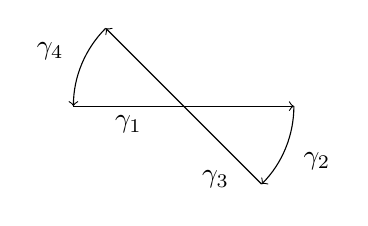
\begin{tikzpicture}[scale=0.7]
\draw[->] (-2,0)--(2,0);
\draw[->] (2,0) arc (0:-45:2);
\draw[->] (1.41421,-1.41421)--(-1.41421,1.41421);
\draw[<-] (-2,0) arc (180:135:2);
\node[below] at (-1,0) {$\gamma_1$};
\node[right] at (2,-1) {$\gamma_2$};
\node[below left] at (1,-1) {$\gamma_3$};
\node[left] at (-2,1) {$\gamma_4$};
\end{tikzpicture}\end{center}
${}$ Then, the problem is to show 
\[\lim_{R\to\oo}I_1=\sqrt{\frac\pi{it}}.\]
\end{frame}

\begin{frame}
\frametitle{3.2. Computation of fundamental solution (3) - estimate of $I_3$}
Since
\begin{align*}
I_3&=\int_{\gamma_3}e^{-itz^2}\,dz\\
&=\int_{\gamma_3}e^{-it(re^{\frac34\pi i})^2}\,d(re^{\frac34\pi i})\\
&=e^{\frac34\pi i}\int_{-R}^Re^{-tr^2}\,dr,
\end{align*}
we have a limit
\[\lim_{R\to\oo}I_3=e^{\frac34\pi i}\sqrt{\frac{\pi}t}=-\sqrt{\frac\pi{it}}.\]
\end{frame}

\begin{frame}
\frametitle{3.2. Computation of fundamental solution (3) - estimate of $I_2$ and $I_4$}
By change of variable, we have
\[I_2=\int_{\gamma_2}e^{-it(Re^{i\theta})^2}\,d(Re^{i\theta})=\int_0^{-\frac14\pi}e^{-itR^2e^{i2\theta}}Rie^{i\theta}\,d\theta\]
and
\[|I_2|\le\int_0^{\frac\pi4}Re^{-tR^2\sin2\theta}\,d\theta.\]
We can do for $|I_4|$ similarly, so
\[|I_2|+|I_4|\le2\int_0^{\frac\pi4}Re^{-tR^2\sin2\theta}\,d\theta=\int_0^{\frac\pi2}Re^{-tR^2\sin\theta}\,d\theta.\]
\end{frame}

\begin{frame}
\frametitle{3.2. Computation of fundamental solution (3) - estimate of $I_2$ and $I_4$}
If we take $\delta=\frac2\pi R^{-\frac32}$ so that $\sin\delta\ge R^{-\frac32}$, then
\begin{align*}
\int_0^\delta Re^{-tR^2\sin\theta}\,d\theta&\le\int_0^\delta R\,d\theta=\frac2\pi\frac1{\sqrt{R}}\to0,\\
\int_\delta^{\frac\pi2}Re^{-tR^2\sin\theta}\,d\theta&=\int_\delta^{\frac\pi2}Re^{-tR^2\sin\delta}\,d\theta\le\frac\pi2Re^{-t\sqrt{R}}\to0
\end{align*}
as $R\to\oo$; $\bigmath\lim_{R\to\oo}|I_2|+|I_4|=0.$\\[1em]
Consequently,
\[\int e^{-it\xi^2}\,d\xi=\lim_{R\to\oo}I_1=-\lim_{R\to\oo}I_3=\sqrt{\frac\pi{it}},\]
\qed
\end{frame}

\begin{frame}
\frametitle{3.3. Representation formula}
Therefore, we showed
\begin{thm}
The fundamental solution of (1) is
\[K(t,x)=\frac1{\sqrt{4\pi it}^d}e^{i\frac{|x|^2}{4t}},\]
where $\sqrt{i}=e^{\frac14\pi i}$.
\end{thm}
\end{frame}

\begin{frame}
\frametitle{3.3. Representation formula}
\begin{thm}
Let $u$ be the solution of (1).
Then,
\[u(t,x)=\frac1{\sqrt{4\pi it}^d}\int u_0(y)e^{i\frac{|x-y|^2}{4t}}\,dy.\]
\end{thm}
This kind of explicit formula of the solution is called \emph{representation formula}.
${}$
\begin{cor}
\[\sup_x|u(t,x)|\le(4\pi t)^{-\frac d2}\int|u_0(x)|\,dx.\]
\end{cor}

\end{frame}




\section{Method II : Oscillatory integral}

\begin{frame}
\frametitle{4.1. Oscillatory integral}
This method is applicable for more generalized cases, such as the Airy equation or the fractional Schr\"odinger equation.\\[1em]
${}$ Note that
\[u(t,x)=K(t,x)*u_0(x).\]
By H\"older's inequality,
\[\|u\|_{L^\oo_x}\le\|K(t,-)\|_{L^\oo_x}\|u_0\|_{L^1}.\]

${}$ We have seen that
\[\hat{K}(t,\xi)=\Fconst e^{-it|\xi|^2}.\]
Fourier transforming,
\[K(t,x)=\frac1{(2\pi)^d}\int e^{i(x\.\xi-t|\xi|^2)}\,d\xi.\]
${}$
We can find this by Fourier transform of complex Gaussian, but we will use another approach.

\end{frame}

\begin{frame}
\frametitle{4.1. Oscillatory integral}
Define \emph{phase} and \emph{amplitude} by
\[\phi(t,x,\xi):=x\.\xi-t|\xi|^2,\qquad a(\xi):=\frac1{(2\pi)^d}\chi(\xi),\]
so that the limit ($\chi\to1$) of the following integral is the fundamental solution:
\[I(t,x):=\int a(\xi)e^{i\phi}\,d\xi.\]
An integral of this form is called \emph{oscillatory integral}.

${}$ We are going to obtain a pointwise estimate of this!$\impl$ Fix $x$.
\end{frame}


\begin{frame}
\frametitle{4.2. Principle of non-stationary phase}
\begin{center}\includegraphics[width=0.8\textwidth]{graph}\end{center}
Where $\del_\xi\phi$ is big, the integral $\int a(\xi)e^{i\phi}\,d\xi$ will be cancelled by oscillation.
\end{frame}


\begin{frame}
\frametitle{4.2. Principle of non-stationary phase}
\begin{defn}
Let $\phi$ be the phase function defined previously.
A \emph{stationary point} is a point $\xi^o(t,x)$ at which $\del_\xi\phi$ vanishes.
\end{defn}
${}$ For the Schr\"odinger equation, we have $\xi^o=\frac x{2t}$.
${}$ The strategy is to divide the integral $I$ as
\[\boxed{I=I_{stat}+I_{nonstat}}\]
${}$
We can control each integral by
\begin{itemize}
\item $I_{stat}$ : base $\x$ height.
\item $I_{nonstat}$ : cancellation by fast oscillation.
\end{itemize}
${}$ The wider the region of stationary phase, the bigger $I_{stat}$ is.\\
${}$ The smaller the region of stationary phase, the bigger $I_{nonstat}$ is.\noindent\\[1em]
${}$ We should find the balance: ${}$ in fact $t^{-\frac 12}$ is the boundary of the regions:
\[I_{stat}\simeq (t^{-\frac12})^d\x1=t^{-\frac d2}.\]
\end{frame}


\begin{frame}
\frametitle{4.3. Heuristic method: Linearization of the phase}
There is a nice heuristic method for finding the boundary\\
(, which we already know it is $t^{-\frac 12}$).\\[1em]
${}$ Let $\xi'=\xi-\xi^o$ be a new variable in the Fourier space.\\
Intuitively, the region of stationary phase is determined as
\[\{\xi':|\phi(\xi)-\phi(\xi^o)|\lesssim2\pi\}.\]
${}$ Since
\begin{align*}
2\pi&\gtrsim|\phi(\xi)-\phi(\xi^o)|\\
&\simeq|\Hess_{\xi^o}(\xi',\xi')|\\
&\simeq t|\xi'|^2,
\end{align*}
${}$ the region of stationary phase is $|\xi'|\lesssim t^{-\frac12}$.
\end{frame}

\begin{frame}
\frametitle{4.4. Repeated integration by parts}
So, the rest is to show $|I_{nonstat}|\lesssim t^{-\frac d2}$, where
\[I_{nonstat}=\int\chi_{|\xi|>t^{-\frac12}}(\xi)a(\xi)e^{i\phi}\,d\xi.\]
By the Taylor expansion
\[\del_\xi\phi=\frac12\Hess_{\xi^o}(\xi')+O(|\xi|^2)=t\xi'+O(|\xi|^2),\]

\end{frame}

\end{document}






